\begin{figure}[!htbp]
\centering
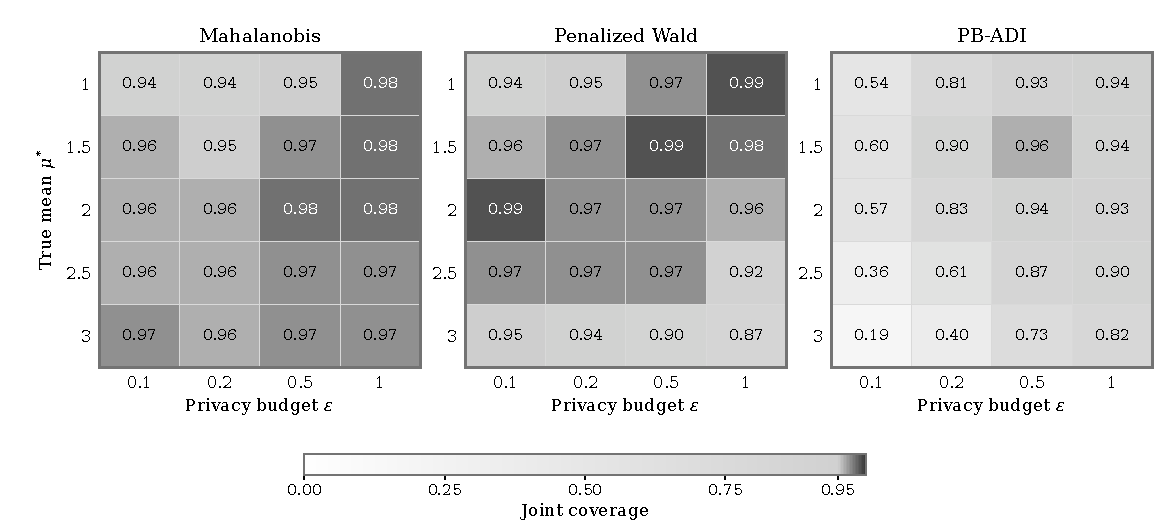
\includegraphics[width=0.95\linewidth]{results/figures/fig_boundary_joint.pdf}
\caption{Joint coverage of the nominal $95\%$ region for $(\mu,\sigma)$ as the true mean approaches the upper clamp $U=3$, at which point the clamp binds on half the sample. Rows are $\mu^\ast$ and columns the privacy budget; the grey scale breaks at $0.95$, so light cells are under-coverage, and the finite-$R$ bound is $0.95025$. Each cell uses $100$ replications, so the Monte Carlo standard error near $0.95$ is $0.022$ and differences below about $0.04$ should not be read as real.}
\label{fig:boundary-joint}
\end{figure}
